\section{Non-inverting Nx Multilevel BC}\label{ch:MBC}

Adding Cockcroft Walton Multiplier explained in Chapter~\ref{ch:cock} with a Conventional Boost Converter (Chapter~\ref{ch:CBC}), we get the Non-inverting Nx Multilevel Boost Converter as shown on Figure~\ref{fig:MBC_CW_CBCtoNx}. \cite{Bhaskar2016}

\begin{figure}[H]
   \centering
   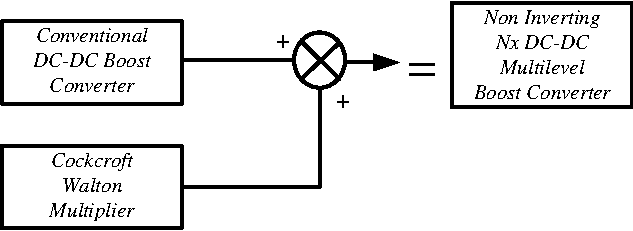
\includegraphics[width=\textwidth]{figures/yMultilevel/CW_CBCtoNx.pdf}
   \caption{Inverting Nx MBC Diagram}
	\label{fig:MBC_CW_CBCtoNx}
\end{figure}


The Non-inverting Nx Multilevel Boost Converter (Figure~\ref{fig:MBC_3XFULL}) is based on one switching device, 2N - 1 diodes and 2N - 1 capacitors, where N indicates the level number of the converter and can be extended by adding capacitors and diodes while the main circuit is not required to be changed. \cite{Rosas-Caro2008}

\begin{figure}[H]
   \centering
   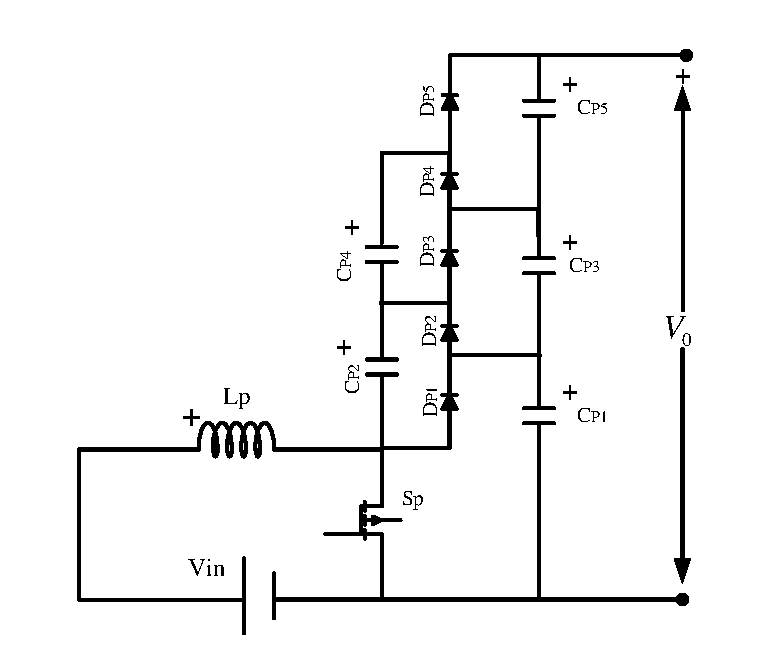
\includegraphics[width=0.9\textwidth]{figures/yMultilevel/3x_FULL.pdf}
    \caption{Nx Multilevel Boost Converter}
	\label{fig:MBC_3XFULL}
\end{figure}

\subsection{Additions from Conventional BC}
The first part of the converter is the conventional DC-DC boost converter described in Chapter~\ref{ch:CBC}. The difference between the two converters is that the output of the multilevel converter is $V_C$ multiplied by the number of levels N, so that a higher output - input voltage ratio can be achieved. The example on Figure~\ref{fig:MBC_3XFULL} is a three-level converter, which means that the output voltage will equal to $3V_{Cp1}$. 

\subsection{Switching States}
The switching modes are the same as a Conventional BC. Like the other topologies mentioned on the previous pages, we assume that the size of all inductors and capacitors is the same. The corresponding circuits for ON and OFF states are displayed on Figure~\ref{fig:MBC_States} and they are based on \cite{Rosas-Caro2008}.

\begin{figure}[H]%
    \centering
    \subfloat[Switch ON\label{MBC_ON}]
    {{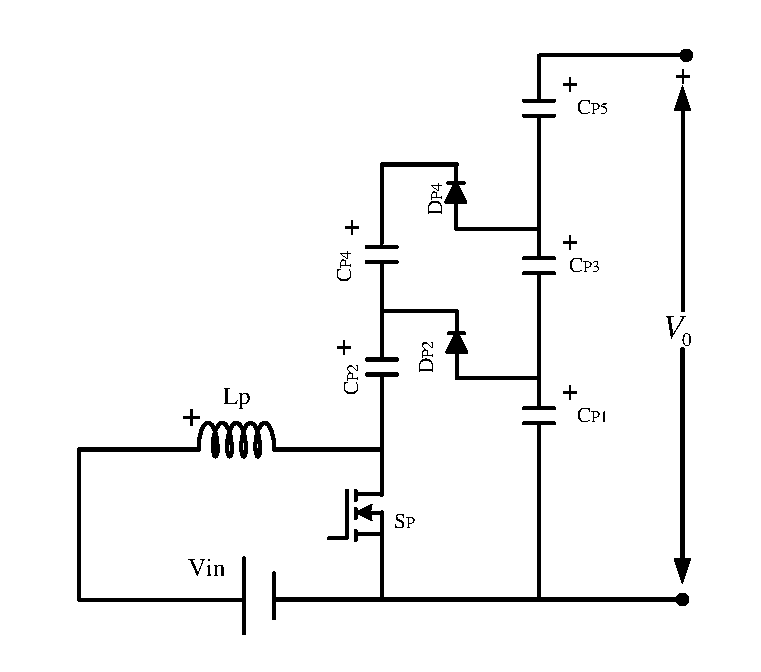
\includegraphics[width=0.45\textwidth]{figures/yMultiLevel/3x_ON.pdf} }}%
    \qquad
    \subfloat[Switch OFF\label{MBC_OFF}]{{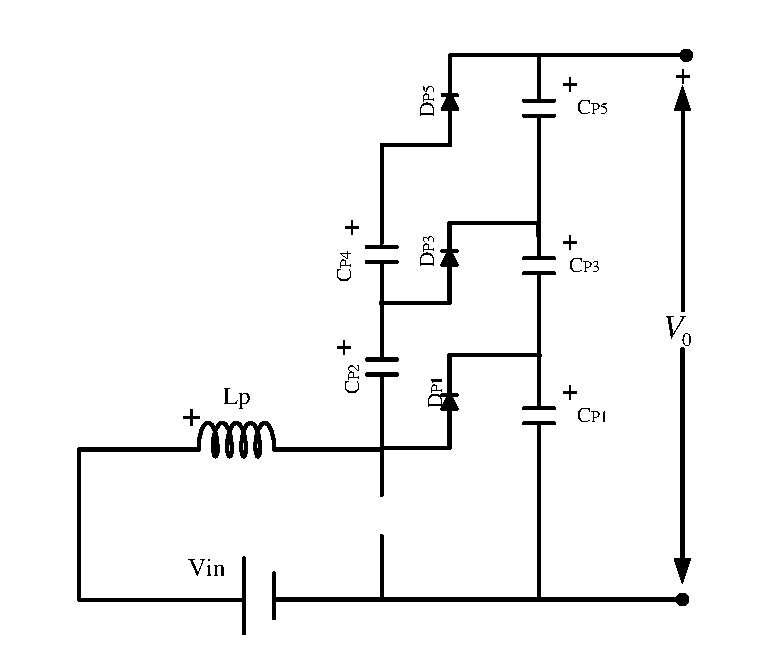
\includegraphics[width=0.45\textwidth]{figures/yMultiLevel/3x_OFF.pdf} }}%  
    \caption{Switching states of the MBC}%
     \label{fig:MBC_States}% 
\end{figure}


\subsubsection{ON State}

During the ON state, $L_p$ is charged by the voltage source. If the voltage across $C_{P1}$ is higher then $C_{P2}$, the capacitor $C_{P1}$ clamps $C_{P2}$ through $D_{P2}$. At the same time, if the voltage across $C_{P2}$ + $C_{P4}$ is smaller than $C_{P1}$ + $C_{P3}$, then the capacitor $C_{P1}$ and $C_{P3}$ clamp the voltage across $C_{P2}$ and $C_{P4}$ through $D_{P4}$ and $C_{P4}$ is clamped by $C_{P3}$. The equations for when the switch is in ON position are as follows:

\begin{equation}
	V_L = V_{in} 
	\label{eq:MBC_ON1}
\end{equation} 

\begin{equation}
	V_{Cp1} = V_{Cp2} = V_{Cp3} = V_{Cp4}
	\label{eq:MBC_ON2}
\end{equation} 

\begin{equation}
	V_{Cp1} + V_{Cp4} = V_{Cp1} + V_{Cp3}
	\label{eq:MBC_ON3}
\end{equation} 

\begin{equation}
	V_o = V_{Cp1} + V_{Cp3} + V_{Cp5} = 3V_{Cp1}
	\label{eq:MBC_ON4}
\end{equation}

\subsubsection{OFF State}
When the switch is open, the inductor is in discharge mode and is charging capacitor $C_{P1}$ through diode $D_{P1}$. At this time $V_{in}$, $V_{Lp}$ and $C_{P2}$ clamp the voltage across $C_{P1}$ and $C_{P3}$ through diode $D_{P3}$. In the same manner, the input voltage $V_{in}$, the inductor voltage $V_{Lp}$, the voltage across $C_{P2}$ and $C_{P4}$ clamp the voltage across $C_{P1}$, $C_{P3}$ and $C_{P5}$.

\vspace{15mm}
The equations for the off state of the switch are as follows:

\begin{equation}
	V_L = V_{in} - V_{Cp1}
	\label{eq:MBC_OFF1}
\end{equation}

\begin{equation}
	V_{Cp1} + V_{Cp3} = V_{in} - V{L} + V_{Cp2}
	\label{eq:MBC_OFF2}
\end{equation}
 
\begin{equation}
	V_{Cp1} + V_{Cp3} + V_{Cp5} = V_{in} - V{L} + V_{Cp2} + V_{Cp4}
	\label{eq:MBC_OFF3}
\end{equation}

\begin{equation}
	V_{Cp1} + V_{Cp3} + V_{Cp5} = V_o
	\label{eq:MBC_OFF4}
\end{equation}

\subsection{Conversion Ratio}

To find the conversion ratio of this converter we can use the Inductor voltage-second balance as follows:

\begin{equation}
	V_{in}D + V_{in}(1-D) - V_{Cp1}(1-D)= 0 
	\Rightarrow
	V_{in} = V_{Cp1}(1-D)
	\label{eq:MBC_INVSB1}
\end{equation}

From Equations~\ref{eq:MBC_ON4} and~\ref{eq:MBC_INVSB1}, output-input voltage relationship is:
\begin{equation}
	\frac{V_o}{V_{in}} = \frac{3V_{Cp1}}{V_{Cp1}(1-D)} = \frac{3}{(1-D)}
	\label{eq:MBC_INVSB2}
\end{equation}

From here, we can generalize the conversion ratio for a Nx Multilevel Boost Converter as:
\begin{equation}
	\frac{V_o}{V_{in}} = \frac{N}{(1-D)}
	\label{eq:MBC_INVSB3}
\end{equation}

\subsection{Simulation results}

To confirm the calculations, the circuit was simulated in SIMULINK, using the following parameters: 

\begin{table}[H]
\begin{center}
\caption {Simulation parameters for MBC} \label{tab:MBC} 
\begin{tabular}{|l|l|}
\cline{1-2}
\textbf{Parameter} & \textbf{Value}  \\ \cline{1-2}
Input Voltage $V_{in}$          &      10V   \\ \cline{1-2}
Load(R)   & 225$\Omega$           \\ \cline{1-2}
Capacitance(C)          &       220$\mu$F     \\ \cline{1-2}
Inductance(L)          &      150$\mu$F      \\ \cline{1-2}
Duty cycle(D)          &     0.6       \\ \cline{1-2}
Switching Frequency($f$)          &      50kHz      \\ \cline{1-2}
\end{tabular}
\end{center}
\end{table}
\vspace{-6mm}
The  topology was modelled with the listed values Figure.\ref{fig:MBC_Sim}. As the previous topologies presented, the components were assumed ideal.
\vspace{-4mm}
\begin{figure}[H]
   \centering
   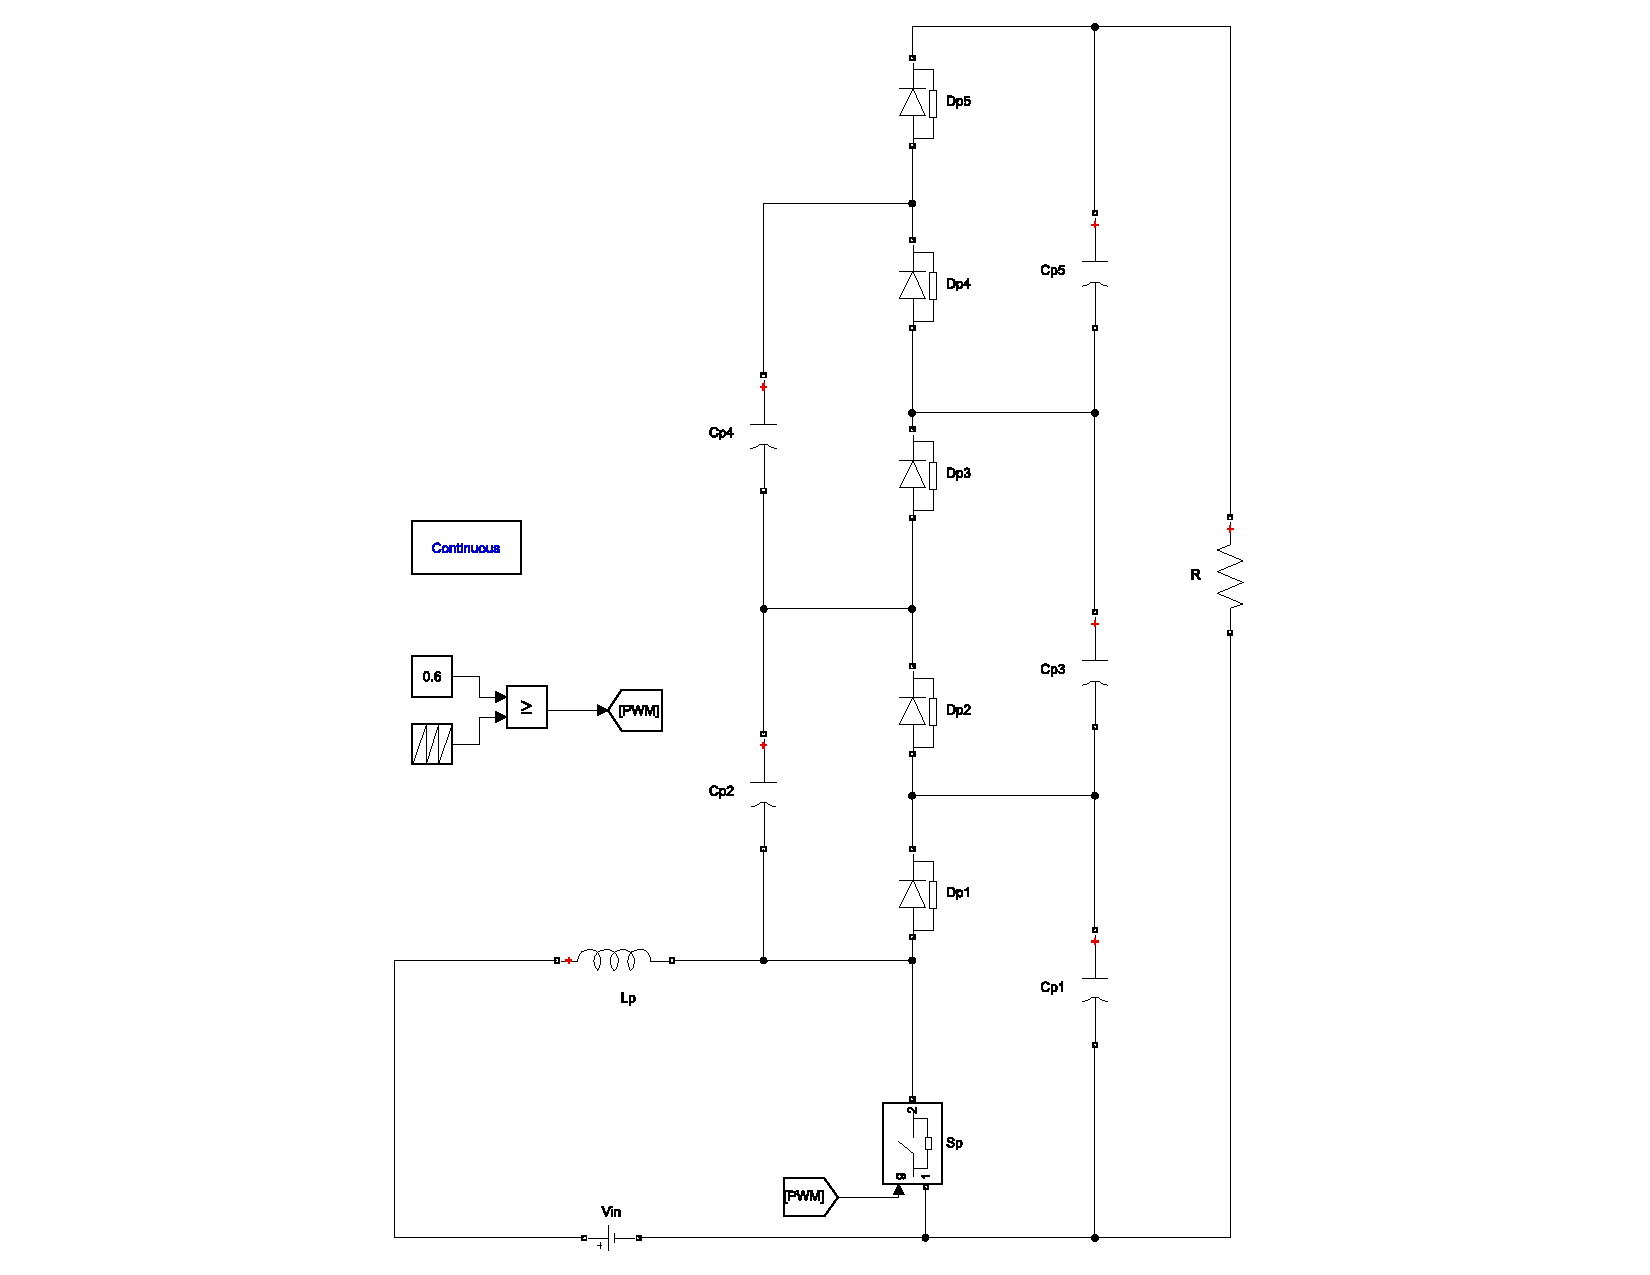
\includegraphics[width=\textwidth]{figures/yMultilevel/MCB_Simulation.pdf}
   \vspace{-4mm}
    \caption{Nx Multilevel Boost Converter Simulation}
	\label{fig:MBC_Sim}
\end{figure}
\vspace{-4mm}
For the three level boost converter, the voltage gain for 0.6 duty cycle is 7.5. Running the simulation, we get the corresponding result of 75V as observed on Figure~\ref{fig:MBC_SimResults}.
\vspace{-2mm}
\begin{figure}[H]
   \centering
   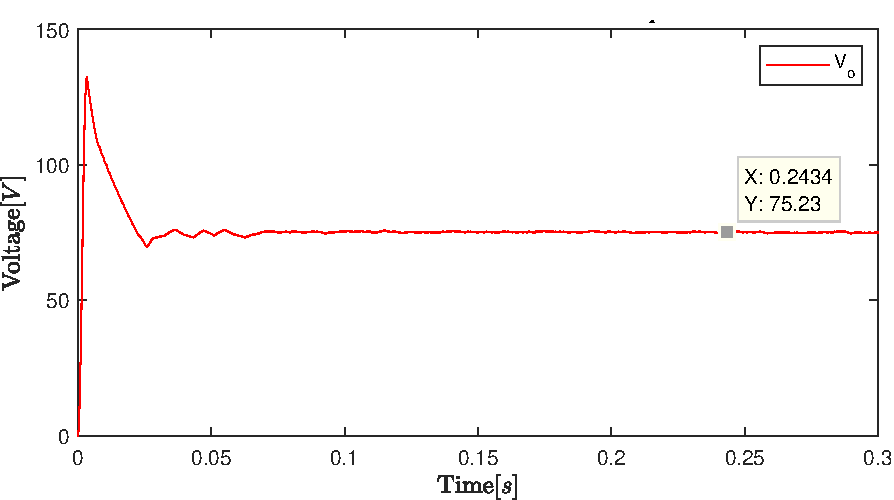
\includegraphics[width=0.8\textwidth]{figures/yMultilevel/Non-invertingNx.pdf}
    \caption{Nx Multilevel Boost Converter Simulation Results}
	\label{fig:MBC_SimResults}
\end{figure}

\section{Inverting Nx Multilevel BC}\label{ch:IMBC}

The Inverting Nx Multilevel Boost Converter can be achieved similar to the non-inverting one, but this time the Cockcroft Walton Multiplier is substracted as shown on Figure~\ref{fig:MBC_CW_CBCtoINx}. \cite{Bhaskar2016}

\begin{figure}[H]
   \centering
   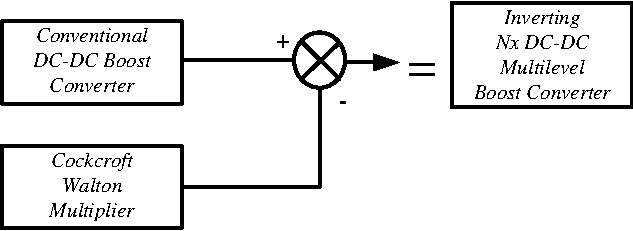
\includegraphics[width=0.8\textwidth]{figures/yMultilevel/InvertingNxDiagram.pdf}
    \caption{Inverting Nx MBC Diagram}
	\label{fig:MBC_CW_CBCtoINx}
\end{figure}
\vspace{-4mm}
The switching states equations and the conversion ratio are not derived as they are the same as the non-inverting Nx Multilevel Boost Converter. The main difference between the two converters is that additional diode and a capacitor are added as well as the diodes are reversed, so that the output voltage becomes with a negative sign as shown on Figure~\ref{fig:MBC_InvertingNx}.
\vspace{-4mm}
\begin{figure}[H]
   \centering
   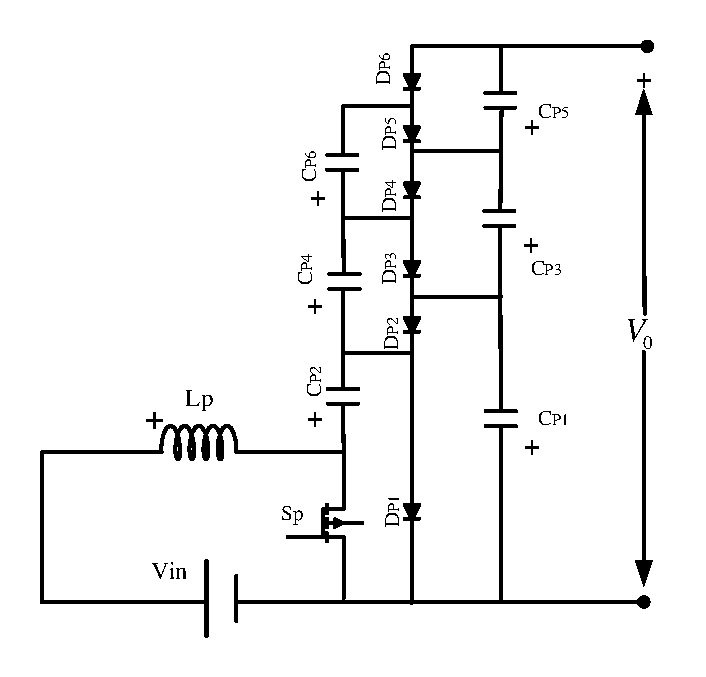
\includegraphics[width=0.7\textwidth]{figures/yMultilevel/InvertingMBCforReport2.pdf}
    \caption{Inverting Nx MBC Schematic}
	\label{fig:MBC_InvertingNx}
\end{figure}

